%!TEX root=main.tex
\section{ClickNP Language}
\label{clicknp:sec:language}

\subsection{Element Graph}

ClickNP script defines a directed graph of elements and channels, which adapts some syntax from the Click modular router \cite{kohler2000click}.

Following ClickNP script and figure \ref{clicknp:fig:ClickNPScriptExample} defines the 网卡-to-ToR part of a network application with NVGRE encapsulation and Per-VM rate limiting.

\begin{figure}[!t]
	\centering
	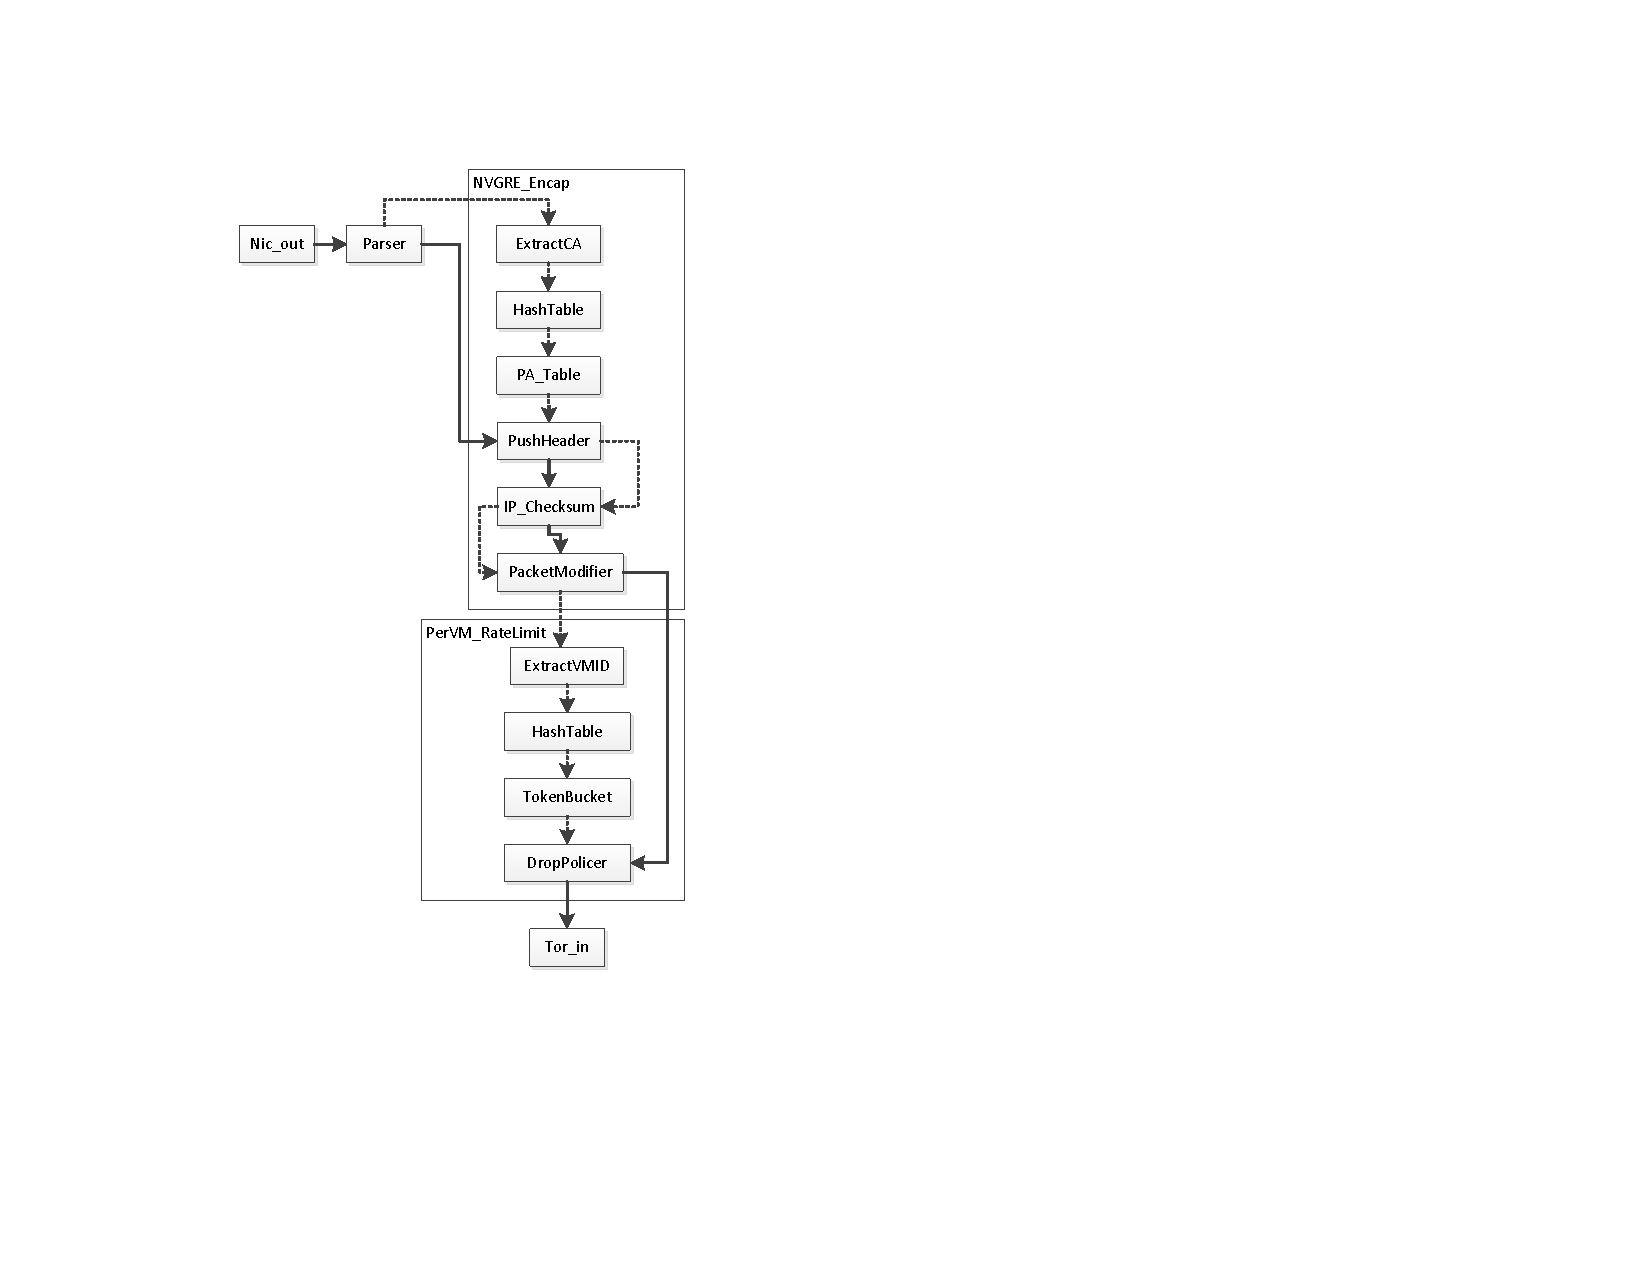
\includegraphics[width=1.0\columnwidth]{image/ApplicationExample}
	\vspace{-0.25in}
	\caption{NVGRE Encap + Rate Limiting in ClickNP}
	\vspace{-0.15in}
	\label{clicknp:fig:ClickNPScriptExample}
	%    
\end{figure}

\begin{lstlisting}
.element_group NVGRE_Encap {
    PushHeader :: encap (2,2)
    begin[1] -> [1]encap -> IP_Checksum (2,2) -> PacketModifer (2,2) -> end
    begin[2] -> ExtractCA (1,1) -> HashTable @ (1,1,14) -> PA_Table @ (1,1) -> [2]encap
}
.element_group PerVM_RateLimit {
    DropPolicer :: action (2,2)
    begin[1] -> [1]action -> end
    begin[2] -> ExtractVMID (1,1) -> HashTable @ (1,1,4) -> TokenBucket @ (1,1) -> [1]action
}
PerVM_RateLimit :: ratelimit (2,2)
nic_out -> Parser (1,2) -> NVGRE_Encap (2,2) -> ratelimit[1] -> tor_in
ratelimit[2] -> Drop (1,0)
\end{lstlisting}

Per clock cycle, each element can read at most one 64-byte message from each input channel and write zero or one 64-byte message to each output channel. A channel either pass \textit{flit} messages (solid line) or \textit{metadata} messages (dotted line). Each flit contains 32 bytes of packet content and flags indicating start of packet (sop) and end of packet (eop). Metadata format is user-defined, containing parsed packet header and optionally a subsequent action.

Lines 1--5 defines an \textit{element group} of 6 elements. Line 2 instantiates a \textit{PushHeader} element with name \textit{encap}. Numbers in parentheses stand for number of input and output ports, and optional subsequent numbers are element parameters (see section \ref{clicknp:subsec:elementdef}). Square brackets indicate the port number to be connected via channel. ``@'' symbol indicates on-the-fly host control.

Metadata containing parsed packet headers flow into the element group via port 1, where Customer Address (CA) is extracted and matched against a \textit{HashTable} controlled by host problem, then the match result is used as the index to Physical Address (PA) table (also controlled by host program). PA table modifies the action part of metadata to contain outer header offset, length and data. Along with packet content flits buffered in channel, metadata is sent to \textit{PushHeader} element where packets actually get shifted. The metadata (with action cleared) and packet flits continue to the \textit{IP\_Checksum} element where new IP header checksum is calculated and a packet modify action is generated to update the IP checksum field in subsequent \textit{PacketModifier} element.

Our initiative for separating flit and metadata messages is not only for clarity but also for performance. One reason is to alleviate the throughput burden of lookup tables. Typically table lookup is done once per packet, while each Ethernet packet has 2--48 flits. If flits are passed through via lookup tables, since we can process at most one flit per cycle, we need to finish each iteration in one cycle in order to reach line rate, but lookup tables which both read and write to local memory need two cycles due to memory timing.

Another reason for flit-metadata separation is to pipeline packet modification actions. For example, in \textit{IP\_Checksum} action, the IP header crosses the boundary of first and second flits, therefore the checksum can only be calculated after the first two flits have arrived. However, the IP checksum field to be updated is in the first flit. If we use one channel for both flit and metadata, then the element has to output nothing in the first cycle processing a packet. As discussed in section \ref{clicknp:subsec:designgoals}, such per-packet idle cycle is unacceptable for our line-rate FPGA implementation. By transferring flit and metadata in separate channels, \textit{IP\_Checksum} element can pass through flits while calculating the checksum, and flits are buffered in the channel between \textit{IP\_Checksum} and \textit{PacketModifier}. When metadata containing IP checksum is received by \textit{PacketModifier}, the first flit is also ready. This coding style eliminates the need for buffers within elements which are more resource hungry than buffers within channels.

A network application is typically built with a parser and a chain of network functions. A network function first builds a lookup key from parsed packet header, match the key in a lookup table (section \ref{clicknp:subsec:lookuptables}), then builds an action based on the match result. The action and packet flits are then passed into an action element. This coding convention allows lookup table elements to be generic, actions to be chained, network functions to be chained and packet parser to be shared.

\subsection{Element Definition}
\label{clicknp:subsec:elementdef}

An element has five components: states, ports, an initializer, a data handler and a signal handler.

\textit{States} define variables that are persistent throughout the lifecycle of an element. Each element has some input and output \textit{ports}, whose number is configured by element graph. \textit{Initializer} is executed once right after the element launches. Main processing loop is composed of a data handler (\textit{.handler}) and a signal handler (\textit{.signal}).

Each element instance with host control enabled (``@'' symbol) will be connected to two special kernels \textit{CmdHub\_in} and \textit{CmdHub\_out}. \textit{CmdHub\_in} is a demux from PCIe input to signal-enabled kernels, \textit{CmdHub\_out} is a mux from signal-enabled kernels to PCIe output. For each iteration, if there is signal input from the host program, the signal will be unmarshaled from PCIe packet to \textit{event}, the signal handler is called, then \textit{outevent} is marshaled to a PCIe packet and sent back to host. Otherwise, input channels are checked for new message, the data handler is called, then output channels are written.

Data handler should check whether or not its input ports have message ready, read states, perform calculation, write back changes to states, optionally write to output ports and return which input ports are to read next iteration. Each input port have a buffer of one message size, and a handler is free to consume or not consume the message by calling or not calling \textit{clear\_input\_ready}. If there are multiple calls to \textit{set\_output\_port} for a same port in one iteration, only the last call will be effective.

The \textit{IP\_Lookup} element below is a binary-tree based IP classifier. The number of nodes per tree level is controlled by the third parameter in element instantiation. The element reads IP address from input port 1, consults the table and writes result to output port 1.

To reduce resource utilization in FPGA, the host program should keep an exact copy of the tree structure, and the assignment of nodes for rule update is handled by host program. The signal handler executes node update instructions from host program. The read interface in signal handler is for crash recovery of host program, so that the restarted host program can rebuild the tree from FPGA.

\begin{lstlisting}
.element IP_Lookup {
    .state {
        // levels of binary tree
        constexpr DEPTH = 32;
        // max entry num per level
        constexpr WIDTH = $3;
        .repeat (depth, 0, DEPTH) {
            constexpr w = ((1<<depth) < WIDTH ? (1<<depth) : WIDTH);
            short value$depth[w];
            short left$depth[w];
            short right$depth[w];
        }
    }
    .init { }
    .handler {
        if ( !input_ready(PORT_1) )
            return PORT_1;
        bool *ip = (bool *) &input_data[1];
        clear_input_ready(PORT_1);

        short pos = 0;
        short result = 0;
        .repeat (depth, 0, DEPTH) {
            result = value$depth[pos];
            if (ip[depth])
                pos = left$depth[pos];
            else
                pos = right$depth[pos];
            if (pos == 0)
                BREAK;
        }
        set_port_output(1, result);
        return PORT_1;
    }
    .signal (uchar cmd, uchar depth, uint pos, uint value, uint left, uint right) {
        uint pos = event.pos;
        .repeat (i, 0, DEPTH) {
          if (i == event.depth)
            switch (event.cmd) {
              case 1: // update
              value$i[pos] = event.value;
              left$i[pos]  = event.left;
              right$i[pos] = event.right;
              break;
              case 2: // read
              outevent.value = value$i[pos];
              outevent.left  = left$i[pos];
              outevent.right = right$i[pos];
              break;
            }
        }
    }
}
\end{lstlisting}

\textit{.repeat (depth, 0, DEPTH)} generates \textit{DEPTH} copies of code with string \textit{\$depth} replaced with 0, 1, 2\ldots \textit{DEPTH}-1. \textit{BREAK} is a special statement to jump to the end of repeated code blocks. Following show the storage regions for variables.

\begin{itemize}
	%\item \textit{counter} is compiled to a register, which is read and written at most once per iteration, and can be done in one cycle.
	%\item \textit{state\_reg} is compiled to an array of registers because all accesses to the array have constant index, after the loop is unrolled. Each register in the array is read and written once per iteration, and also can be done in one cycle.
	\item State arrays \textit{value}n, \textit{left}n and \textit{right}n are compiled to (3 * \textit{DEPTH}) SRAM blocks. Each array is read (in handler) or written (in signal) once per iteration, so the element can be fully pipelined.
	%\item \textit{Param} is a pointer to global memory. Access to global memory is the bottleneck of the while loop.
	\item Local variables \textit{ip}, \textit{pos} and \textit{result} are intermediate variables in the combinational logic and will occupy no storage space on FPGA.
	\item Loop control variables \textit{depth} and \textit{i}, as well as \textit{constexpr}s, are syntactic sugar for code generation.
\end{itemize}

The tree lookup logic in lines 23--31 is automatically pipelined by ClickNP toolchain. After data flow analysis, variables \textit{pos} and \textit{result} are each split into multiple variables in single static assignment (SSA) form. Since SRAM read has one cycle latency, the lookup will take at least \textit{DEPTH} cycles. Fortunately, these memory read operations can be pipelined. A pipeline with \textit{DEPTH} stages is inferred, each stage holds a copy of live variables \textit{ip}, \textit{pos} and \textit{result} in registers. Different stages of the pipeline processes different copies of live variables (i.e. different copies of input data) simultaneously. Pipelining improves throughput by exploiting temporal parallelism.

The tree update logic in lines 41--43 are independent, so the three memory writes are performed in parallel, which improves throughput by exploiting spatial parallelism.

\subsection{Host Communications}

Signal handler is a stop-and-wait mechanism for host-to-kernel communication. Kernels also need to initiate communications, for example to send alerts, dump packets and use host memory as cache. We develop a streaming interface for kernels to communicate with host program via channels as if host program was another kernel. To use the streaming host interface, an element connects to \textit{host\_in} pseudo-element for input and \textit{host\_out} for output.

ClickNP compiler generates a C++ class for each element type, including 5 methods:
\begin{itemize}
	\item \textit{launch}, launches the corresponding kernel.
	\item \textit{signal}, marshals parameters, send an event to the signal handler, wait to receive outevent and unmarshals the response.
	\item \textit{send}, send a message to kernel via streaming interface.
	\item \textit{receive}, receive a message (block or non-block) to kernel via streaming interface.
	\item \textit{setCallback}, if set, the callback function will be called every time a message is received via streaming interface.
\end{itemize}

The C++ class can be extended to add more methods with clearer semantics. For example, \textit{IP\_Lookup} class provides methods \textit{addRule}, \textit{deleteRule}, \textit{clearTable} and \textit{reloadTable} to encapsulate internal states of the IP lookup tree and a series of node update operations needed for one rule update.

All element classes share a common base class \textit{Element}, and ClickNP compiler generates a \textit{std::map} of element names and element class instances. A host program should first initialize the platform, then execute the \textit{launch} method of each element object.
